\documentclass[a4paper]{article}
\usepackage[T1]{fontenc}
\usepackage[utf8]{inputenc}
\usepackage[italian]{babel}
\usepackage{lipsum}
\usepackage{graphicx}
\author{Anis Lico \and Simone Del Gatto}
\title{Programmazione di reti - Relazione Assigment 1}
\begin{document}
\maketitle
\tableofcontents

\section{Task 1}
\subsection{Netcat}
Come prima cosa è stato consultato il manuale della bash. Netcat viene presentato come un semplice applicativo che consente di inviare una porzione di testo da un host all'altro (oppure sullo stesso host) utilizzando il terminale. L'applicativo comporta l'esecuzione in due modalità principali: come agente che invia i messaggi (client) o come agente che li riceve (server). Eseguendo nella prima modalità si scrive una porzione di testo da inviare sul terminale e premendo \emph{Invio} la si spedisce. Nella modalità di ricevente una volta arrivato il pacchetto viene stampata sullo schermo la scritta ricevuta. 
Per soddisfare la consegna sono state aperti due terminali e sono stati eseguiti i seguenti comandi:
\begin{itemize}
\item \textbf{Client}: \newline
Comando: nc -u 127.0.0.1 1234
Con il flag \emph{-u} si utilizzano per la comunicazione delle socket UDP. Indicando l'indirizzo ip \emph{127.0.0.1} si indica che si vuole inviare allo stesso host su cui si sta eseguendo Netcat.\emph{1234} è invece la porta tramite la quale avviene la comunicazione.
\item \textbf{Server}: \newline
Comando: nc -u -l 127.0.0.1 1234
Nessun parametro differente dal comando precedente tranne \emph{-l} che significa \emph{listen}. Indica perciò che l'applicativo rimarrà \emph{in ascolto} e quindi fungerà da Server
\end{itemize}
Per catturare i messaggi tramite Wireshark è stato eseguito il programma sull'interfaccia \emph{loopback} e filtrando il traffico con \emph{"ip.addr == 127.0.0.1 and udp.port == 1234"}.
\begin{figure}[ht!]
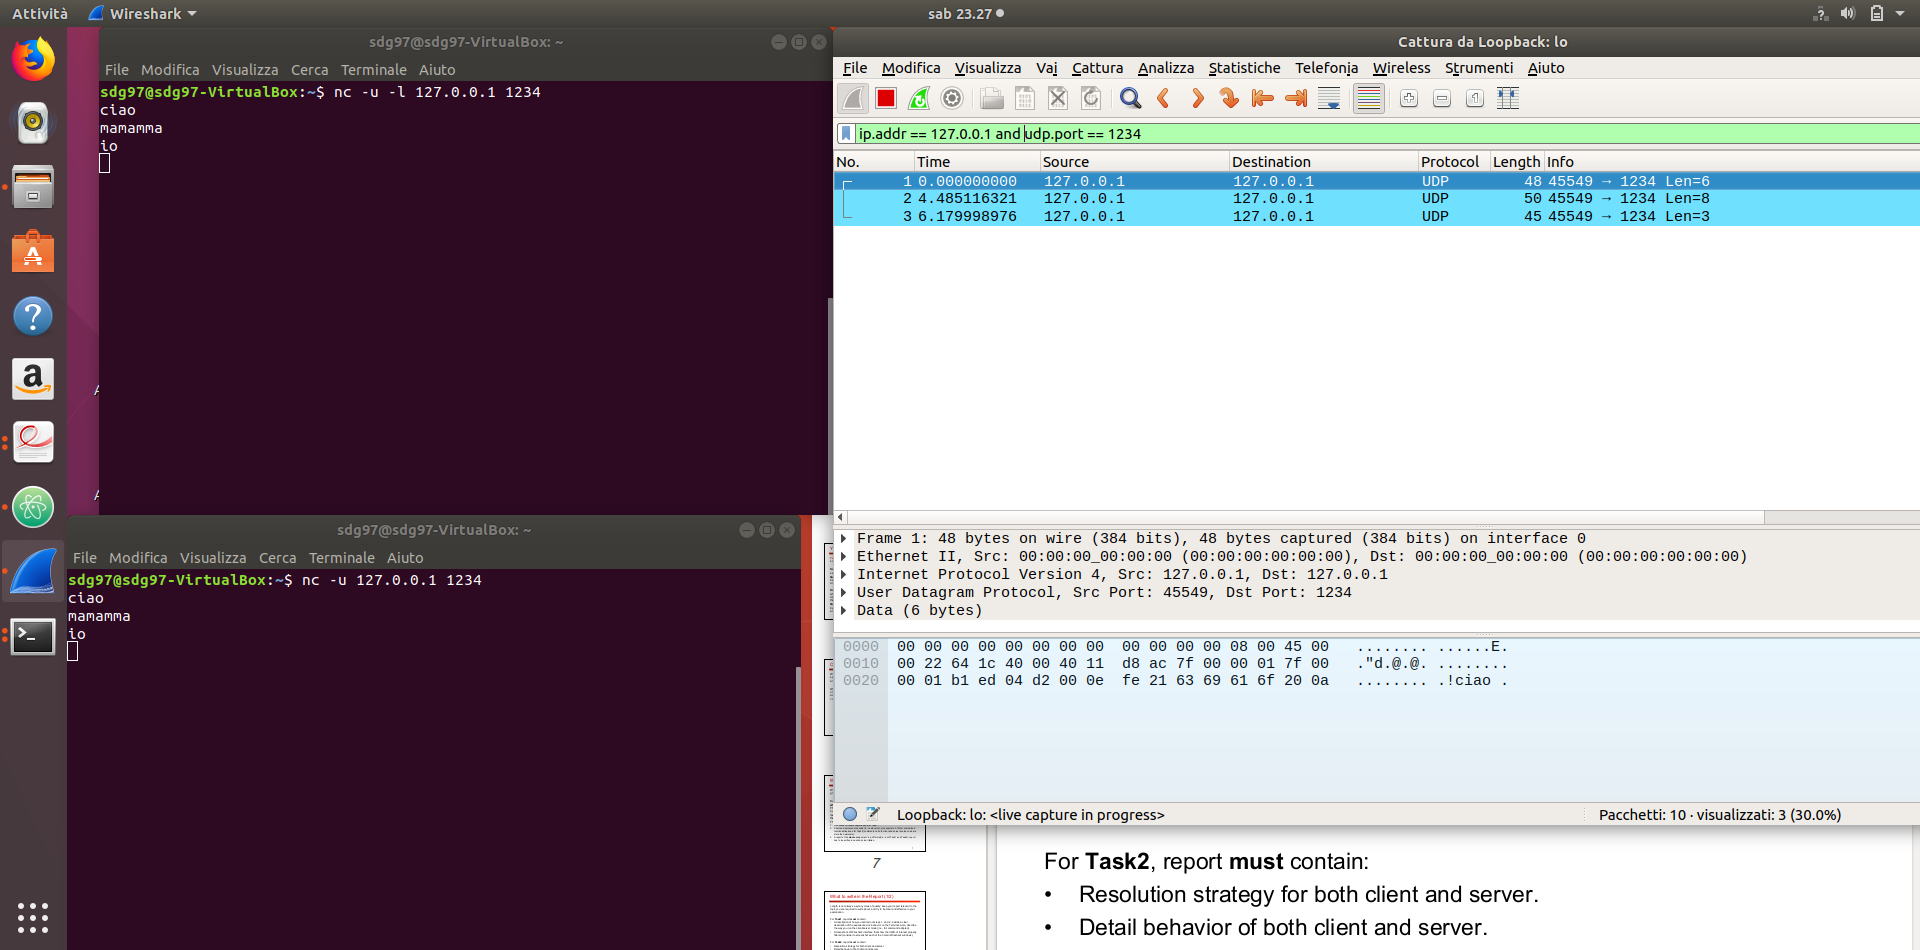
\includegraphics[scale = 0.20]{wireshark.png}
\caption{Schermata di cattura con Wireshark}
\end{figure}

\section{Task 2}
Per implementare il comportamento di Netcat come richiesto abbiamo diviso il codice in due sorgenti distinti, uno per il Client e uno per il Server e abbiamo riadattato il codice visto in classe. Le comunicazioni avvengono come richiesto utilizzando delle socket UDP.
\subsection{Server}
All'inizio dell'esecuzione il Server chiede l'indirizzo ip e la porta che sui quali mettersi in ascolto. Una volta ricevuto un pacchetto stampa le informazioni del client dal quale lo ha ricevute e stampa la stringa che gli è arrivata. Se la stringa corrisponde a\emph{"exit"} allora il server invia al client la stringa \emph{"goodbye"}, stampa a sua volta la string \emph{"goodbye"} e si rimette in ascolto. 
\subsection{Client}
Come il server anche il client chiede all'utente i parametri necessari per poter comunicare (porta e indirizzo ip). Successivamente invita l'utente a scrivere una stringa e inviarla. Se la stringa inviata è \emph{"exit"} il client si mette in ascolto e attende una risposta del Server. Quando il server gli invia il messaggio \emph{"goodbye"} il client stampa a video la stringa \emph{"sever said goodbye"} e termina l'esecuzione.

\begin{figure}[]
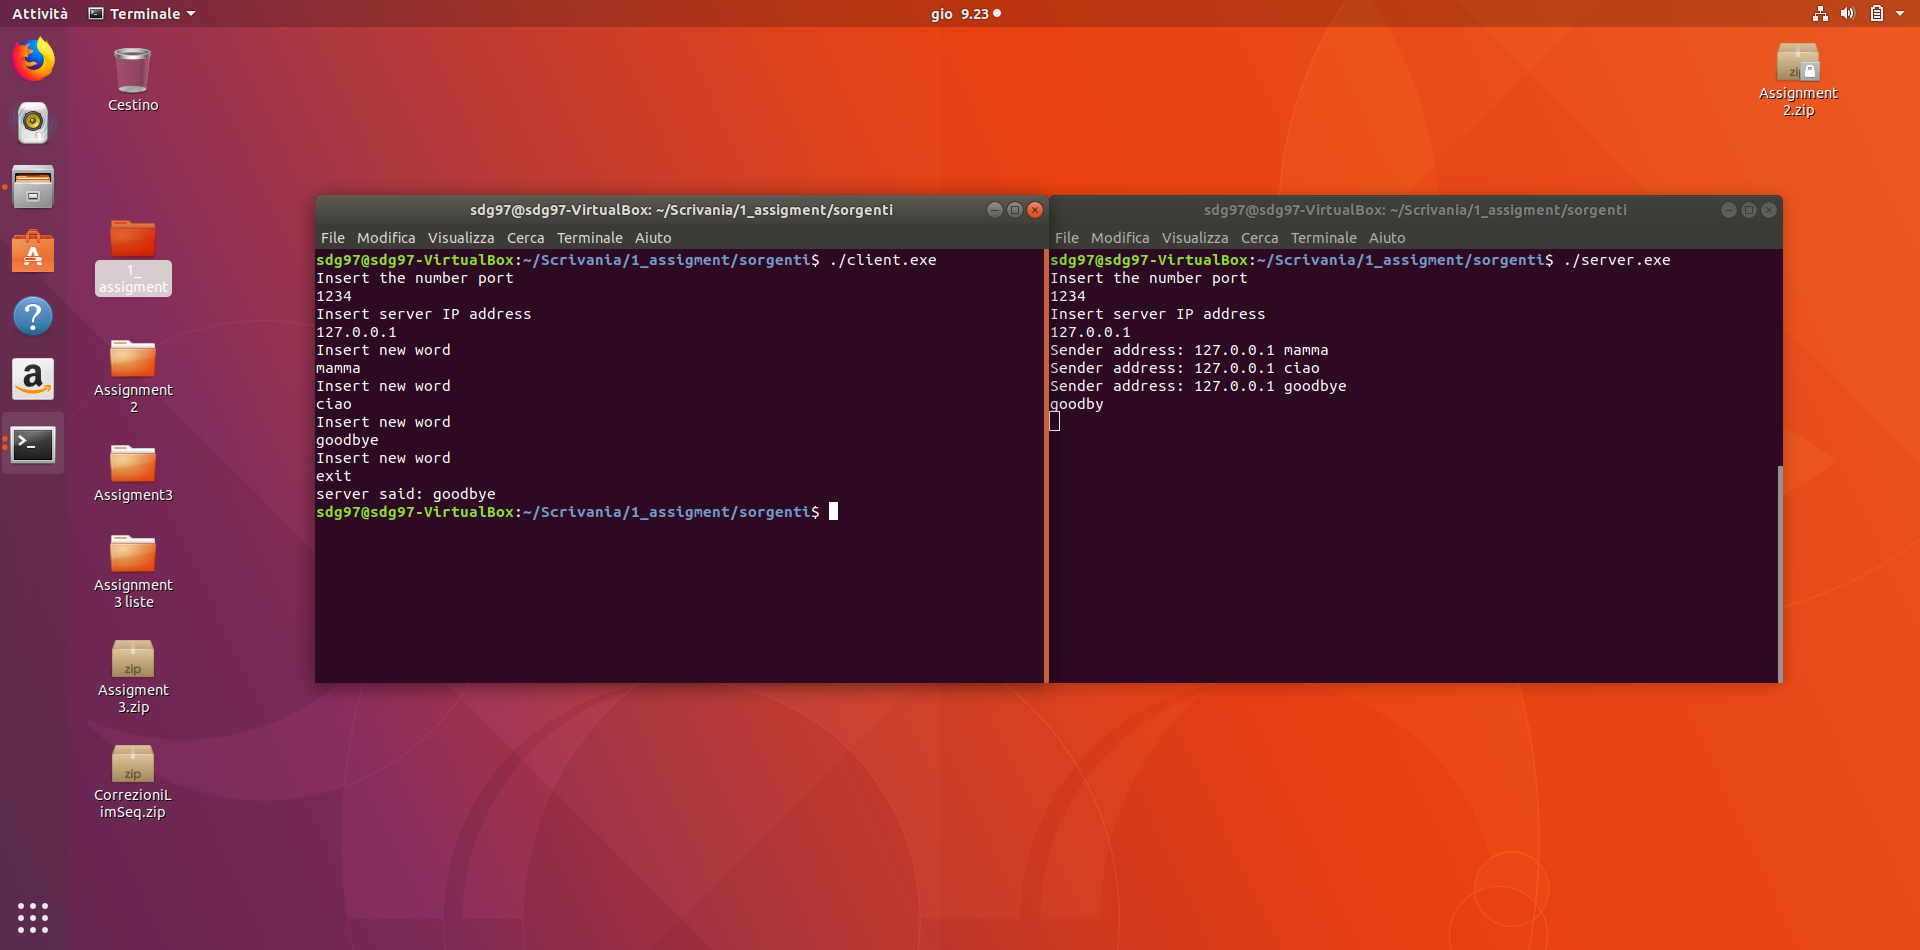
\includegraphics[scale = 0.30]{ClientServerDaMeSviluppati.png}
\centering
\caption{Esempio di esecuzione dei programmi da noi implementati}
\end{figure}
\newpage
\section{Task 3}
\subsection{Scenario 1}
Lanciando due istanze client e un server il comportamento tra i due sembra concorrente.
\subsection{Scenario 2}
Aggiungendo una sleep il comportamento del server di definisce chiaramente come un comportamento di tipo 
sequenziale.
\subsection{Possibile soluzione}
Si potrebbe provare a lavorare con i thread. Se ne utilizza uno che rimane in ascolto sulla porta e per ogni nuovo client che tenta di comunicare con il server viene fatto partire un nuovo thread che gestirà autonomamente la comunicazione con quel client. Il thread poi sarà chiuso quando viene interrotta la connessione. Sarebbe in tal caso necessario trovare un modo affinché un client che ha già precedentemente intrapreso la comunicazione con il server sia reindirizzato verso il thread corretto e non ne venga invece aperto un altro.
\end{document}